\section{Técnicas de Clasificación}

Como hemos visto en el apartado de EDA, tenemos un conjunto desbalanceado. Por la descripción del problema, cometemos un error mayor cuando clasificamos mal la clase Yes. Por tanto, se podría considerar penalizar más los falsos negativos, de manera que los algoritmos de clasificación intenten cometer menores errores de este tipo. 

\subsection{Algoritmo KNN}

Recordamos los gráficos 1-1 con las clasificaciones, vistos en el EDA.

\begin{figure}[H]\center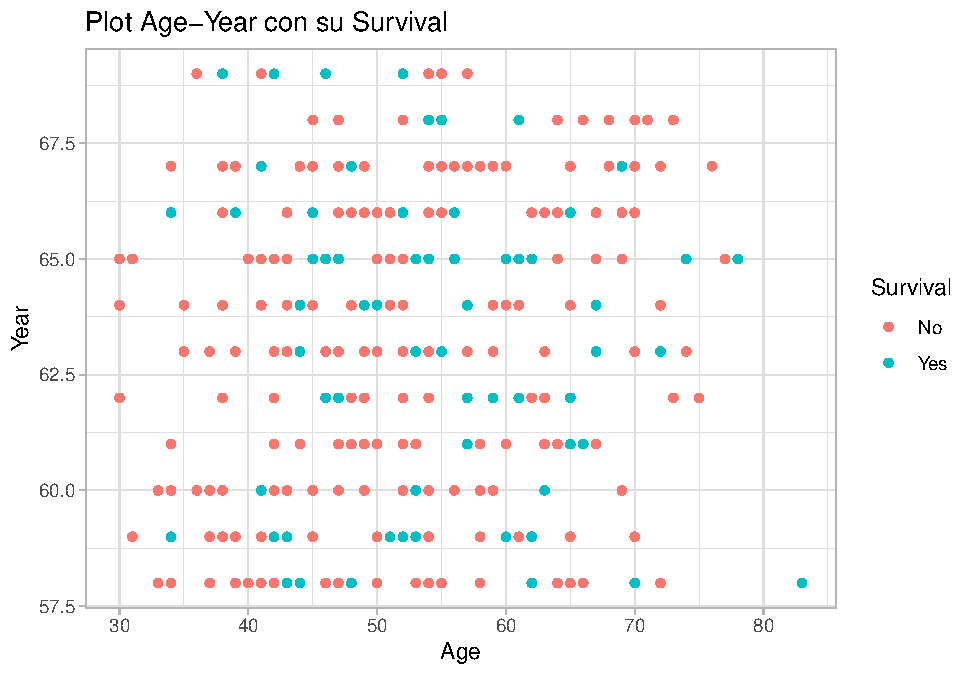
\includegraphics[width=.9\linewidth]{img/Clasificacion_files/figure-latex/unnamed-chunk-7-1}\caption{}\end{figure}

\begin{figure}[H]\center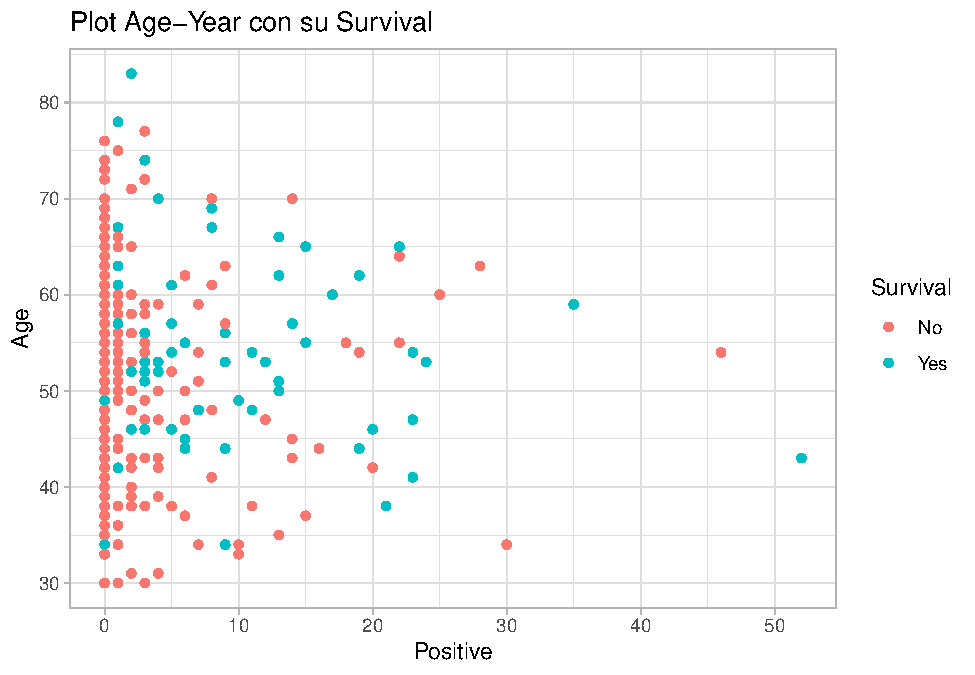
\includegraphics[width=.9\linewidth]{img/Clasificacion_files/figure-latex/unnamed-chunk-7-2}\caption{}\end{figure}

\begin{figure}[H]\center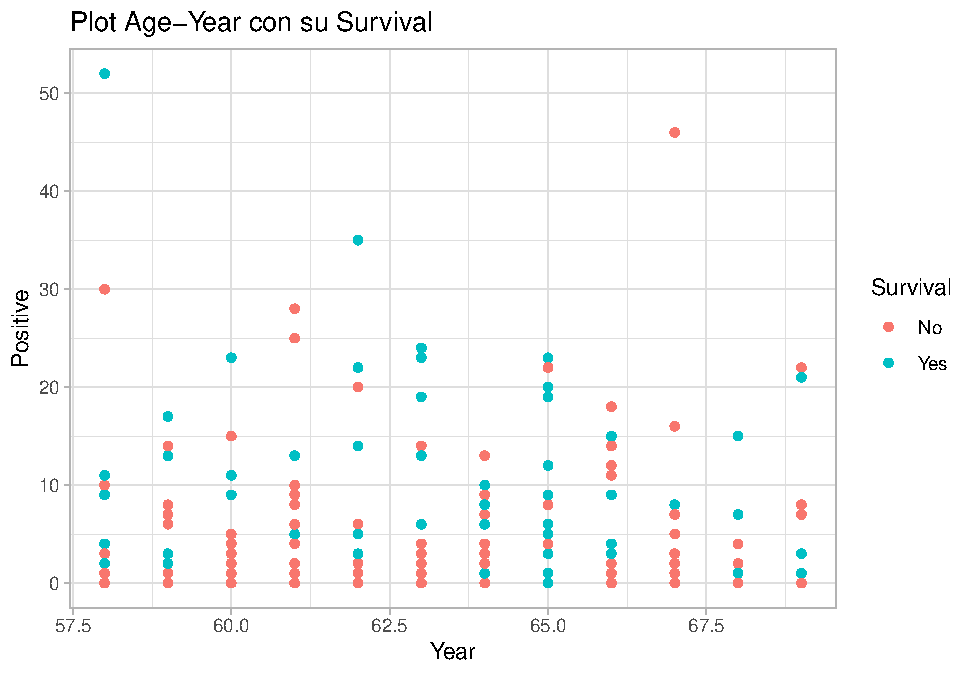
\includegraphics[width=.9\linewidth]{img/Clasificacion_files/figure-latex/unnamed-chunk-7-3}\caption{}\end{figure}

\begin{figure}[H]\center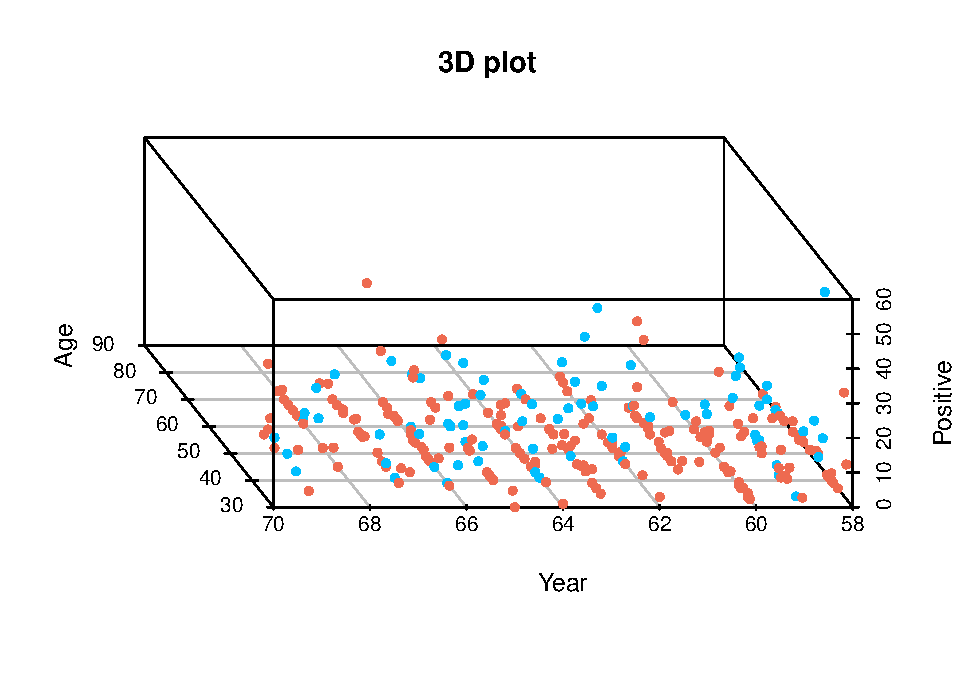
\includegraphics[width=.9\linewidth]{img/Clasificacion_files/figure-latex/unnamed-chunk-8-1}\caption{}\end{figure}

\begin{figure}[H]\center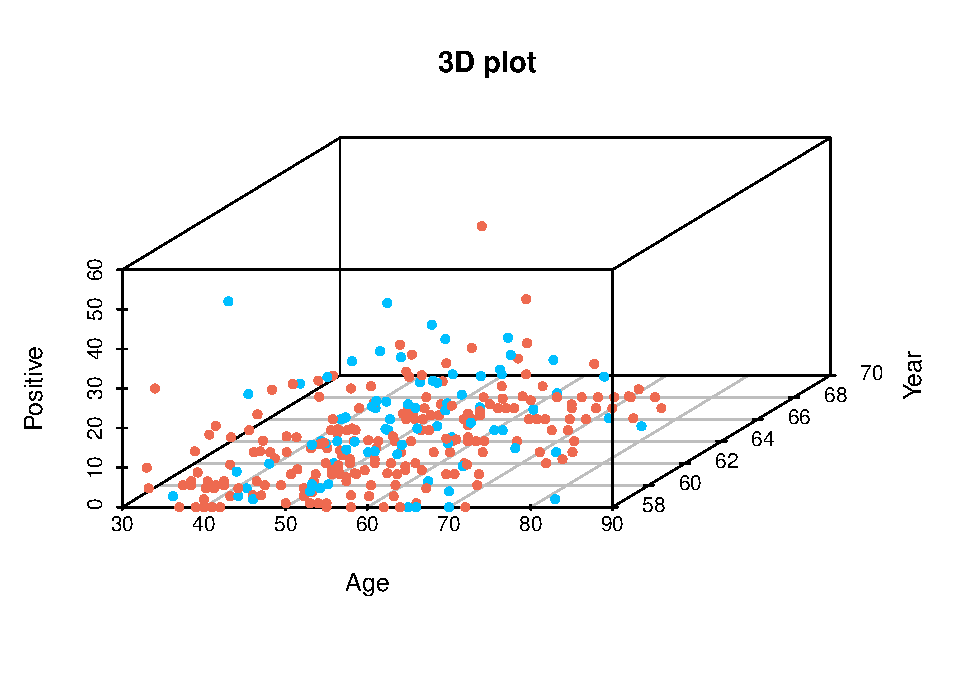
\includegraphics[width=.9\linewidth]{img/Clasificacion_files/figure-latex/unnamed-chunk-8-2}\caption{}\end{figure}

De cara a un algoritmo KNN, apreciamos los datos muy entremezclados, con mayor tendencia a agruparse los no supervivientes que los que sí, pero nada en especial que nos llame la atención.

\vspace{\baselineskip}

Debido a esto vamos a empezar con un valor de K relativamente bajo y vamos a ir aumentándolo poco a poco. Tenemos que tener en cuenta que un K mayor puede ocasionar overfitting, pero usando técnicas de cross-validation podemos minimizar las posibilidades.

Los resultados usando el paquete caret son los siguientes\footnote{Los datos han sido preprocesados con una estandarización antes de aplicar cualquiera de los algoritmos}:
\begin{verbatim}
k-Nearest Neighbors 

275 samples
  3 predictor
  2 classes: 'No', 'Yes' 

No pre-processing
Resampling: Cross-Validated (10 fold) 
Summary of sample sizes: 248, 247, 247, 247, 247, 247, ... 
Resampling results across tuning parameters:

  k   Accuracy   Kappa    
   3  0.6947599  0.2034939
   4  0.6832418  0.1615034
   5  0.6884412  0.1100164
   6  0.6879121  0.1426382
   7  0.6950549  0.0983539
   8  0.7165954  0.1496547
   9  0.7240130  0.1881672
  10  0.7164632  0.1470534
  11  0.7277269  0.1753847
  12  0.7203195  0.1708068
  13  0.7241656  0.1767408
  14  0.7313085  0.2015352
  15  0.7422873  0.2320214

Accuracy was used to select the optimal model using the largest value.
The final value used for the model was k = 15.
\end{verbatim}

\begin{figure}[H]\center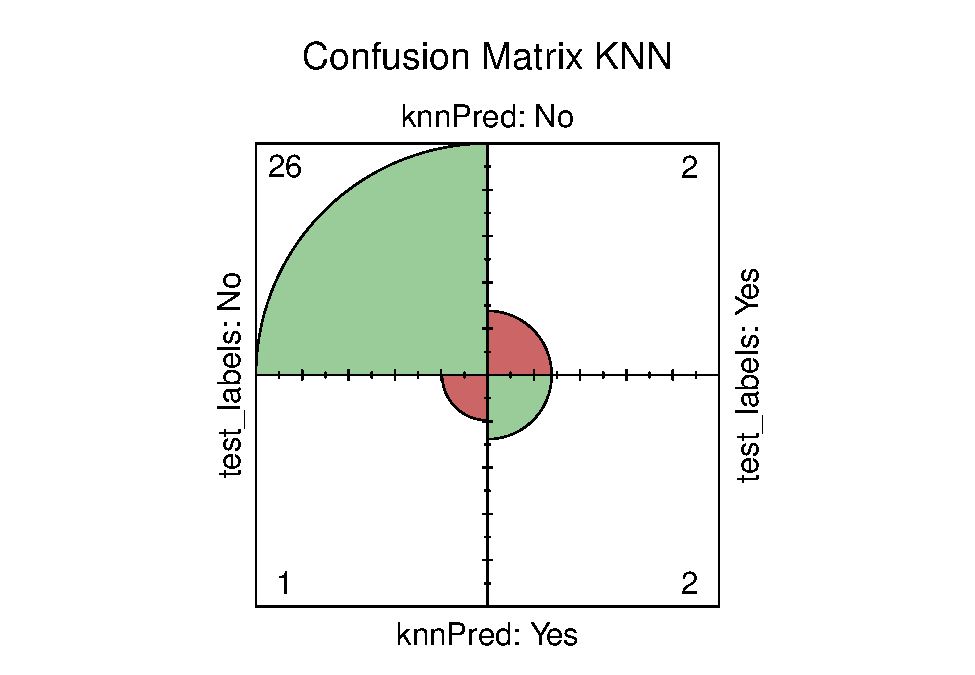
\includegraphics[width=.9\linewidth]{img/Clasificacion_files/figure-latex/unnamed-chunk-11-1}\caption{}\end{figure}

Vemos que al estar los datos tan entremezclados ni siquiera con un K pequeño aprende bien, es ya con un K medianamente alto (= 15) donde obtiene mayor accuracy en train.

Una vez más probablemente esto se deba a la gran mezcla de los datos, de forma que necesite la ``opinión'' de un gran número de vecinos para poder predecir con mayor confianza el nuevo valor.

\begin{figure}[H]\center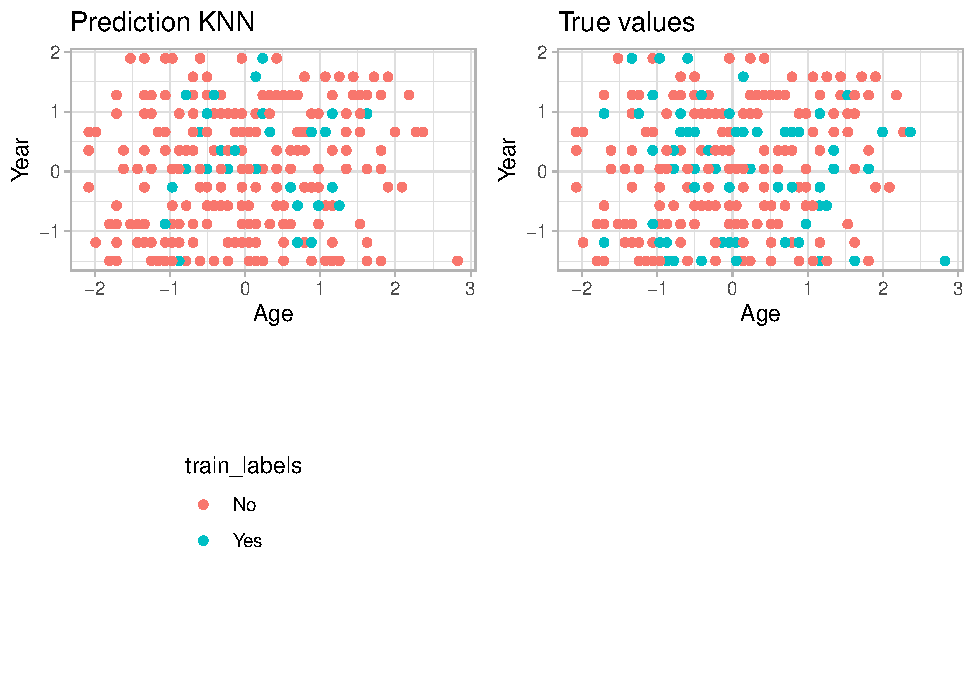
\includegraphics[width=.9\linewidth]{img/Clasificacion_files/figure-latex/unnamed-chunk-12-1}\caption{Predicción con K=15 en training}\end{figure}

Vemos que el uso de un K alto hace que perdamos puntos de Yes. Probablemente al ser minoría el error cometido clasificándolos como No es menor y por eso obtiene mejor accuracy.

\vspace{\baselineskip}

Una evaluación con el subconjunto reservado inicialmente como test nos muestra una calidad extrañamente superior que la de training.

\begin{verbatim}
Test evaluation:
 Accuracy     Kappa 
0.9032258 0.5181347 

Confusion matrix:
knnPred No Yes
    No  26   2
    Yes  1   2
\end{verbatim}

Este comportamiento no es el habitual en aprendizaje automático, parece que casualmente el conjunto de test es bastante fácil de ajustar y por eso se obtienen mejores resultados que en training.
En la sección ?? se muestran las etiquetas. También se vuelve a incidir en la alta presencia de etiquetas \textit{No}.

El valor alto de K hace que se prediga con mayor facilidad este valor de etiqueta y por ese desbalanceo se obtengan tan buenos resultados. En sí es un poco preocupante de cara a la población real de los datos, pero debemos suponer que la muestra que tenemos es representativa y por tanto válida.

Por otro lado, para el problema que nos atañe quizás esto podría ser incluso un hecho positivo, ya que los falsos positivos sería algo que querríamos evitar a toda costa.

\vspace{\baselineskip}

Por comparar, podemos también evaluar con otros valores de K en test. Puesto que hemos obtenido los mejores resultados en training con un K de 15, que es un valor relativamente alto, podemos probar con uno bajo y uno intermedio (3 y 7).

\begin{verbatim}
k-Nearest Neighbors

No pre-processing
Resampling: Cross-Validated (10 fold) 
Summary of sample sizes: 248, 247, 248, 248, 247, 247, ... 
Resampling results:

  Accuracy  Kappa    
  0.697619  0.1988554

Tuning parameter 'k' was held constant at a value of 3
\end{verbatim}

\begin{figure}[H]\center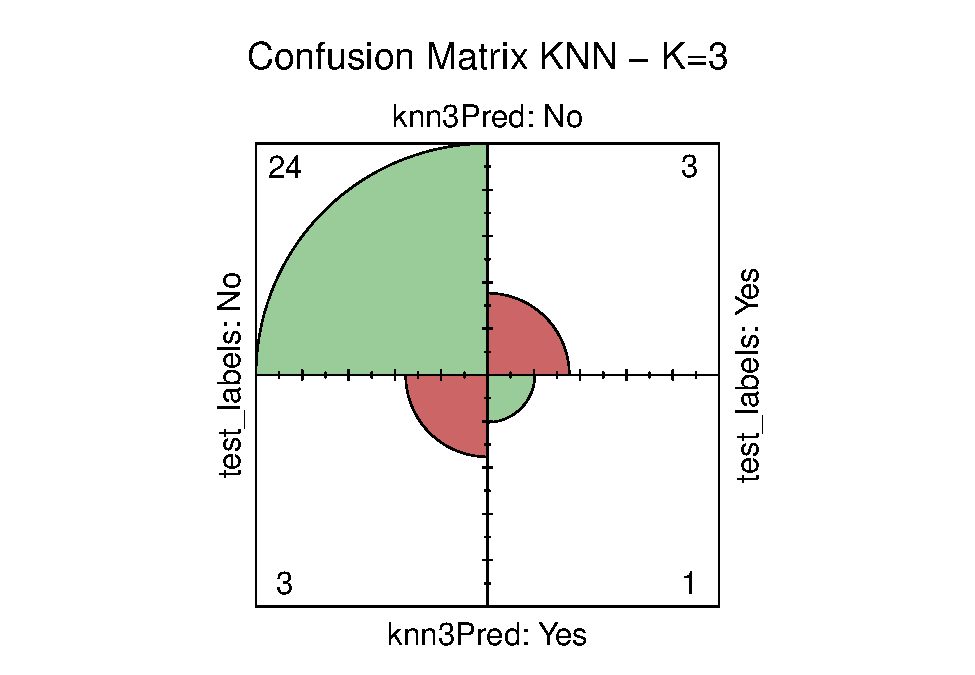
\includegraphics[width=.9\linewidth]{img/Clasificacion_files/figure-latex/unnamed-chunk-14-1}\caption{}\end{figure}

\begin{verbatim}
Test evaluation:
Accuracy     Kappa 
0.8064516 0.1388889

Confusion matrix:
         test_labels
knn3Pred   No Yes
     No    24   3
     Yes    3   1
\end{verbatim}

\begin{verbatim}
k-Nearest Neighbors 

No pre-processing
Resampling: Cross-Validated (10 fold) 
Summary of sample sizes: 248, 247, 247, 248, 248, 247, ... 
Resampling results:

  Accuracy   Kappa     
  0.6761905  0.08141897

Tuning parameter 'k' was held constant at a value of 7
\end{verbatim}

\begin{figure}[H]\center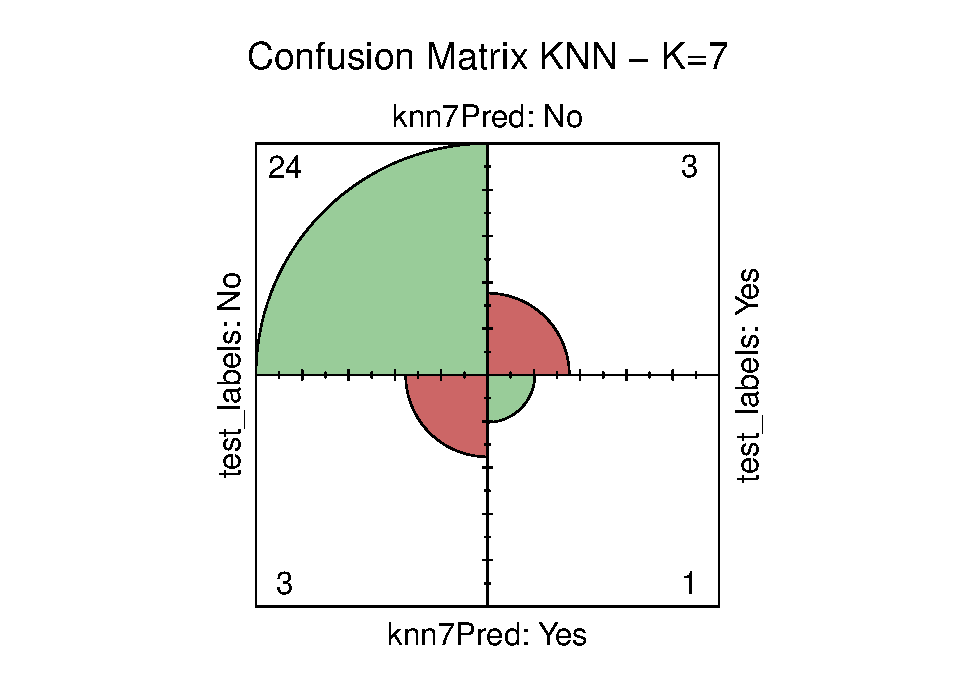
\includegraphics[width=.9\linewidth]{img/Clasificacion_files/figure-latex/unnamed-chunk-16-1}\caption{}\end{figure}

\begin{verbatim}
Test evaluation:
Accuracy     Kappa 
0.8064516 0.1388889

Confusion matrix:
        test_labels
knn7Pred No Yes
     No  24   3
     Yes  3   1 
\end{verbatim}

K=7 vemos que es el que más sufre al evaluar en test, y ambos (tal y como nos había indicado la primera ejecución con CV) tienen una calidad bastante inferior (tanto en training como en test) a un K=15.

\subsection{Algoritmo LDA}
\subsubsection{Asunciones}
Comprobamos asunciones:
\begin{enumerate}
    \item \textbf{Distribución aleatoria}: No nos queda más remedio que creer que sí.
    \item \textbf{Cada predictor sigue una distribución normal}: Ya vimos en el EDA que esto no era cierto. El test de Shapiro nos aseguraba que no había normalidad y los QQ-plots nos lo hacían ver claramente. Técnicamente sabiendo esto no deberíamos usar LDA, pero puesto que esto es un proyecto seguimos.
    
    Por otro lado, las variables Age y Year no parecen seguir una distribución demasiado ``rara'' (en comparación con una normal), por lo que es posible que obtengamos resultados de calidad aceptable.
    \item \textbf{Las clases siguen la misma matriz de covarianza}: Lo comprobamos a continuación.
\end{enumerate}

Calculamos la diagonal de la matriz de correlación para cada una de las clases, obteniendo:
\begin{verbatim}
Para clase Yes:
      Age      Year  Positive 
0.9176155 1.0113109 1.6788033 

Para clase No:
      Age      Year  Positive 
1.0756415 0.9752581 0.5448553 
\end{verbatim}

\vspace{\baselineskip}

Estos valores nos parecen indicar que las variables Age y Positive parecen seguir distintas varianzas, pero es preferible asegurarlo con un test estadístico.

Puesto que nuestras variables no siguen una distribución normal, no podemos hacer el test de homogeneidad de Barlett. Utilizamos por tanto el de Levene
\begin{verbatim}
Age:
\end{verbatim}

\begin{tabular}{l|r|r|r}
\hline
  & Df & F value & Pr(>F)\\
\hline
group & 1 & 1.799898 & 0.1807261\\
\hline
 & 304 &  & \\
\hline
\end{tabular}

\begin{verbatim}
Year:
\end{verbatim}

\begin{tabular}{l|r|r|r}
\hline
  & Df & F value & Pr(>F)\\
\hline
group & 1 & 0.0624405 & 0.8028481\\
\hline
 & 304 &  & \\
\hline
\end{tabular}

\begin{verbatim}
Positive:
\end{verbatim}

\begin{tabular}{l|r|r|r}
\hline
  & Df & F value & Pr(>F)\\
\hline
group & 1 & 18.78912 & 1.99e-05\\
\hline
 & 304 &  & \\
\hline
\end{tabular}

Indicándonos que solo se puede asegurar que la variable Positive no tiene homogeneidad entre clases diferentes.

\vspace{\baselineskip}

Gráficamente:

\begin{figure}[H]\center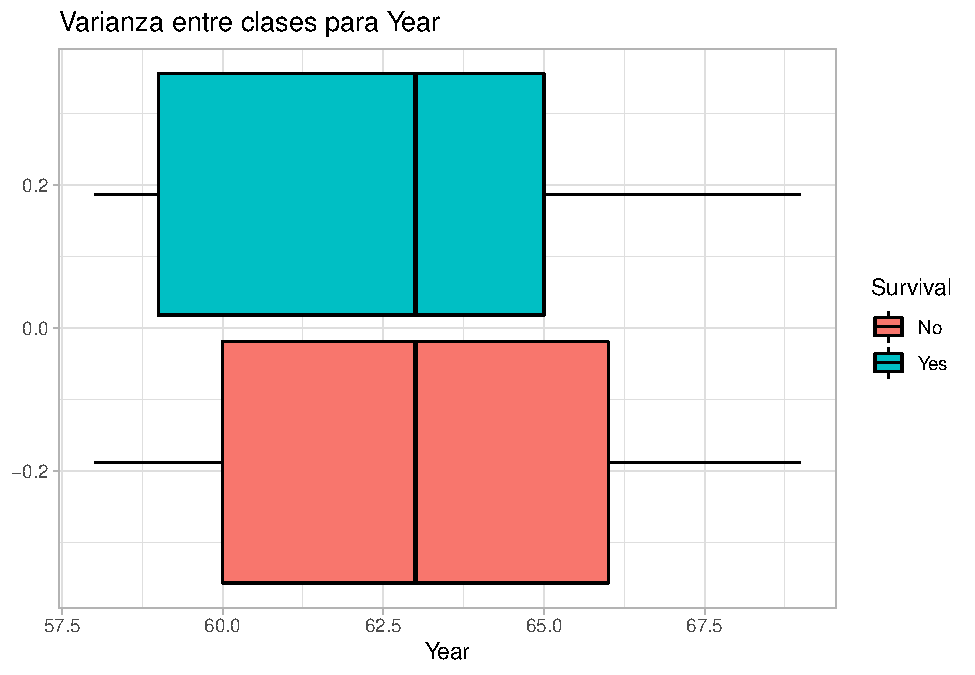
\includegraphics[width=.8\linewidth]{img/Clasificacion_files/figure-latex/unnamed-chunk-19-1}\caption{}\end{figure}

\begin{figure}[H]\center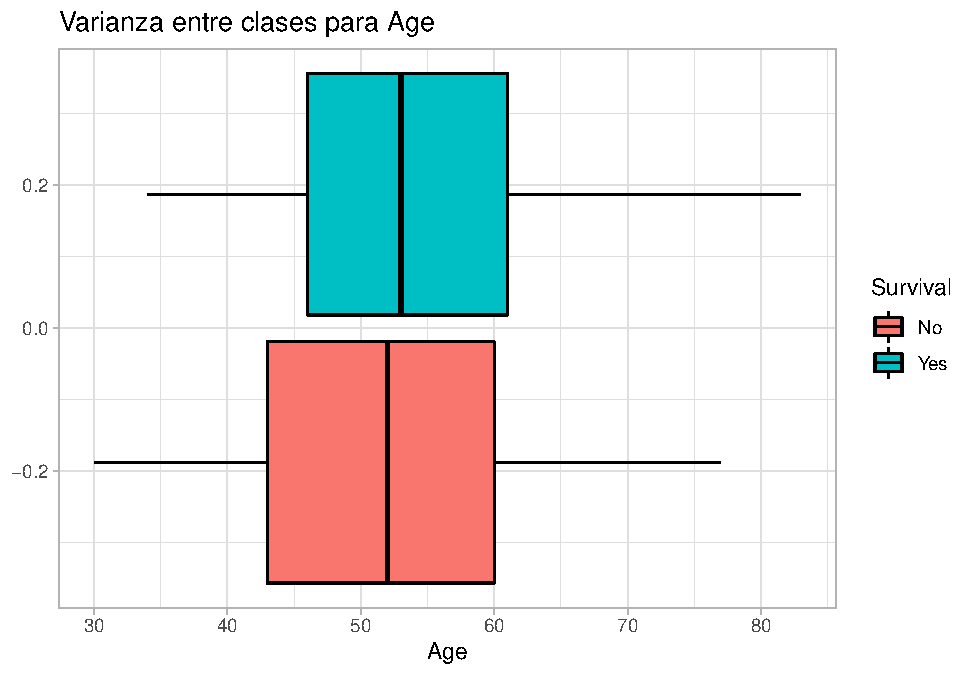
\includegraphics[width=.8\linewidth]{img/Clasificacion_files/figure-latex/unnamed-chunk-19-2}\caption{}\end{figure}

\begin{figure}[H]\center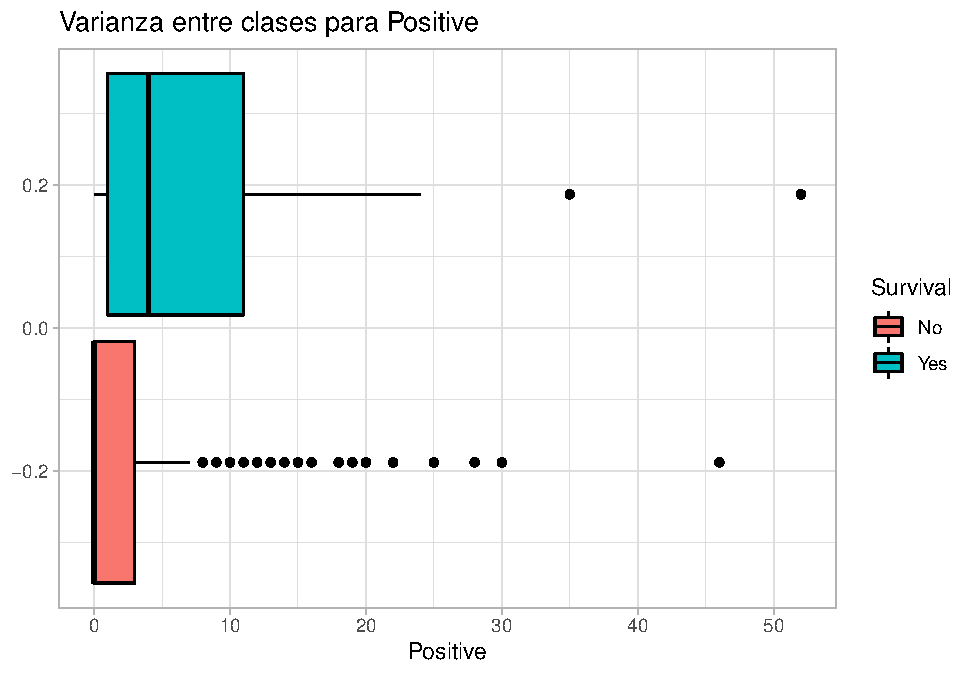
\includegraphics[width=.8\linewidth]{img/Clasificacion_files/figure-latex/unnamed-chunk-19-3}\caption{}\end{figure}

\begin{figure}[H]\center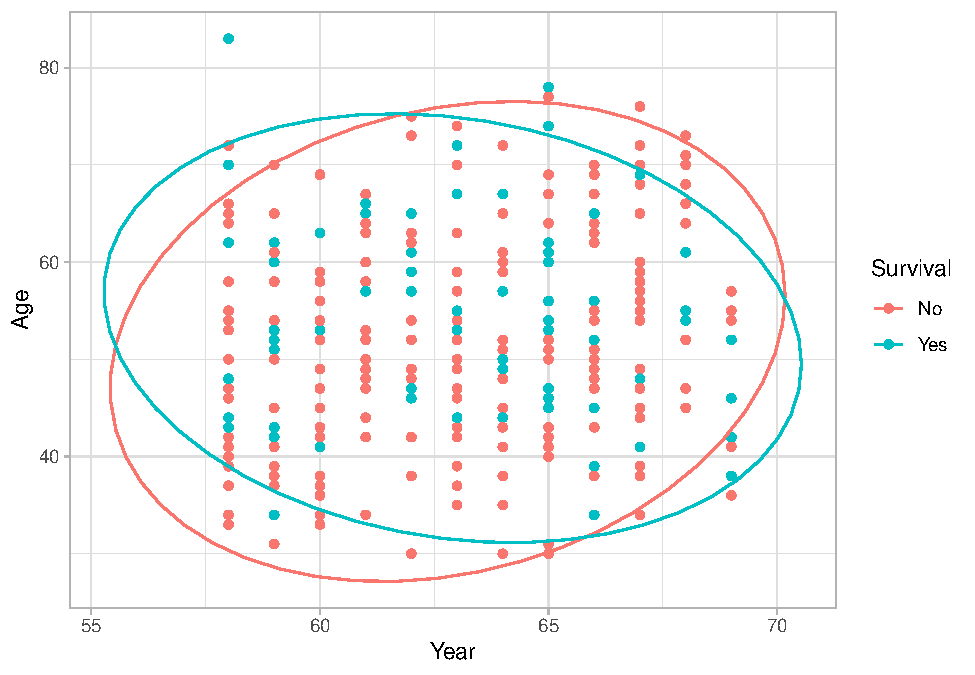
\includegraphics[width=.8\linewidth]{img/Clasificacion_files/figure-latex/unnamed-chunk-20-1}\caption{}\end{figure}

\begin{figure}[H]\center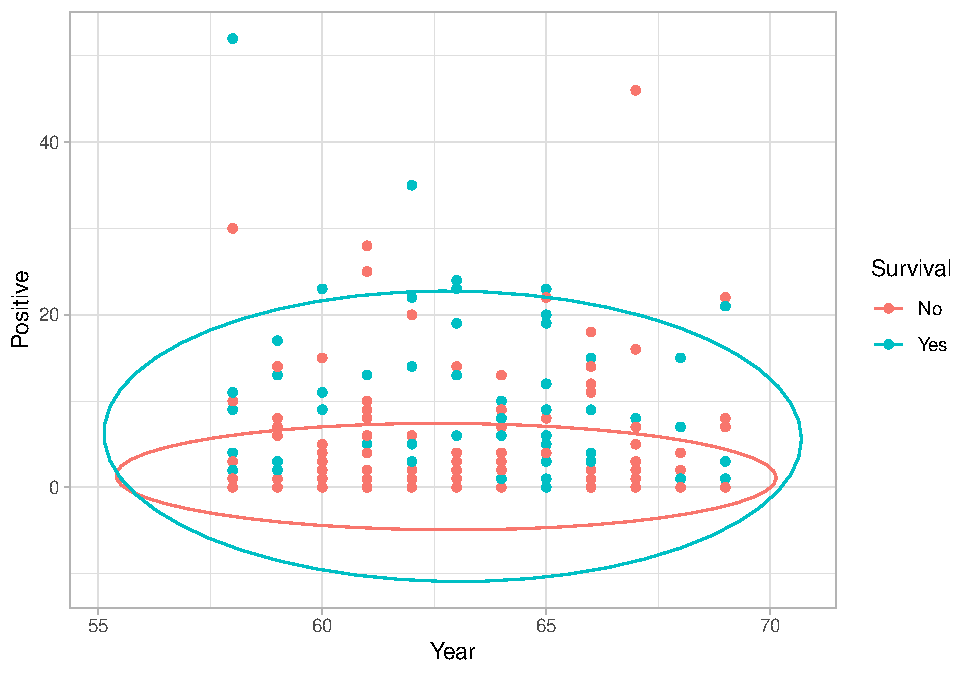
\includegraphics[width=.8\linewidth]{img/Clasificacion_files/figure-latex/unnamed-chunk-20-2}\caption{}\end{figure}

\begin{figure}[H]\center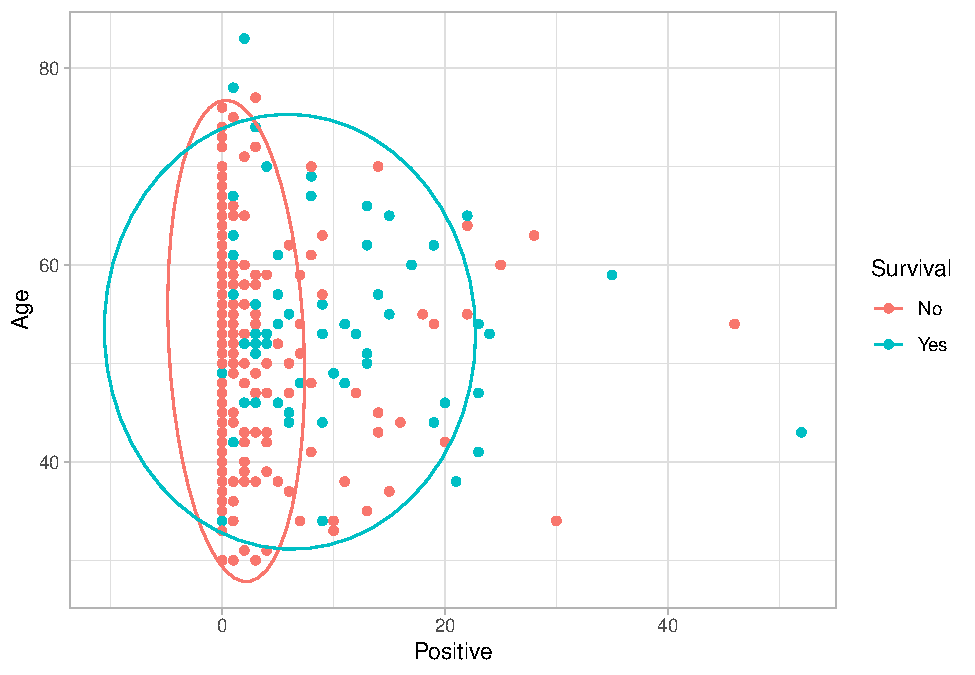
\includegraphics[width=.8\linewidth]{img/Clasificacion_files/figure-latex/unnamed-chunk-20-3}\caption{}\end{figure}

Se nota que la causa de que no se rechace el test para esta variable es la gran cantidad de datos con Positive igual a 0.

\vspace{\baselineskip}

Por tanto para LDA no podemos hacer uso de la variable Positive, puesto que además de la falta de normalidad se incumpliría la asunción número 3, por lo que usamos las otras dos.

\vspace{\baselineskip}

Aunque solo es recomendable, y no son cualidades necesarias para obtener solución en LDA:
\begin{itemize}
    \item Tenemos más instancias que predictores, por varios órdenes de magnitud.
    \item Los predictores son independientes. 
    \item No tenemos varianza cercana a cero.
\end{itemize}

\subsubsection{Aplicación del algoritmo LDA}

\begin{verbatim}
Call:
lda(x, y)

Prior probabilities of groups:
  No  Yes 
0.72 0.28 

Group means:
            Age        Year
No  -0.04141411 0.004845716
Yes  0.11031976 0.021276742

Coefficients of linear discriminants:
            LD1
Age  0.98140853
Year 0.03411981
Cross-Validated (10 fold) Confusion Matrix 

(entries are percentual average cell counts across resamples)
 
          Reference
Prediction No Yes
       No  72  28
       Yes  0   0
                          
 Accuracy (average) : 0.72
\end{verbatim}

\begin{figure}[H]\center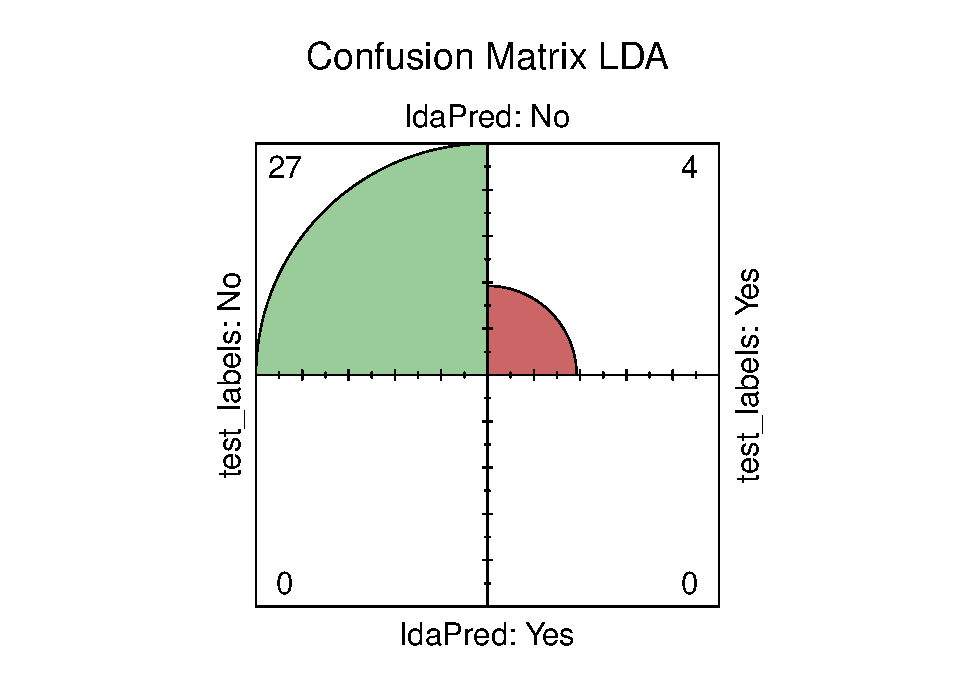
\includegraphics[width=.9\linewidth]{img/Clasificacion_files/figure-latex/unnamed-chunk-23-1}\caption{}\end{figure}

\begin{figure}[H]\center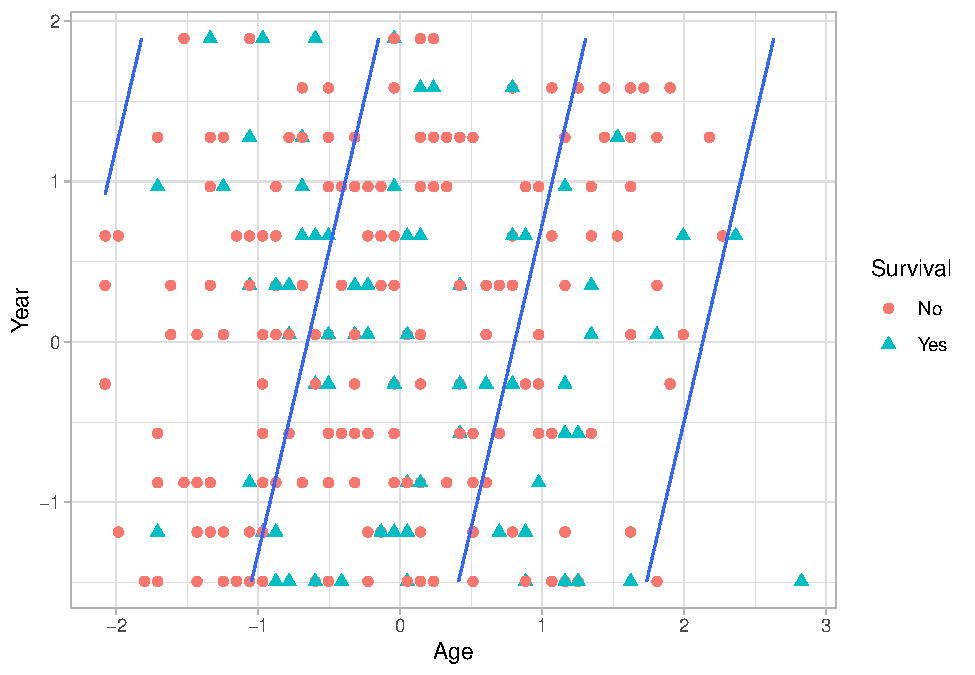
\includegraphics[width=.9\linewidth]{img/Clasificacion_files/figure-latex/unnamed-chunk-24-1}\caption{Predicciones LDA sobre training}\end{figure}

Hacemos un plot del ajuste

\begin{figure}[H]\center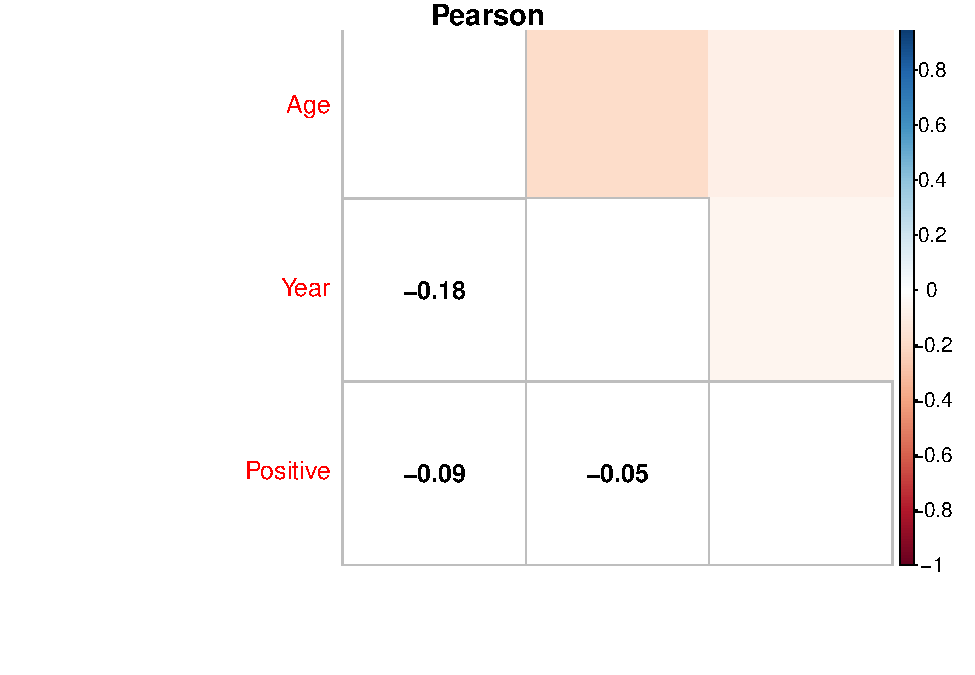
\includegraphics[width=.9\linewidth]{img/Clasificacion_files/figure-latex/unnamed-chunk-25-1}\caption{}\end{figure}

\begin{figure}[H]\center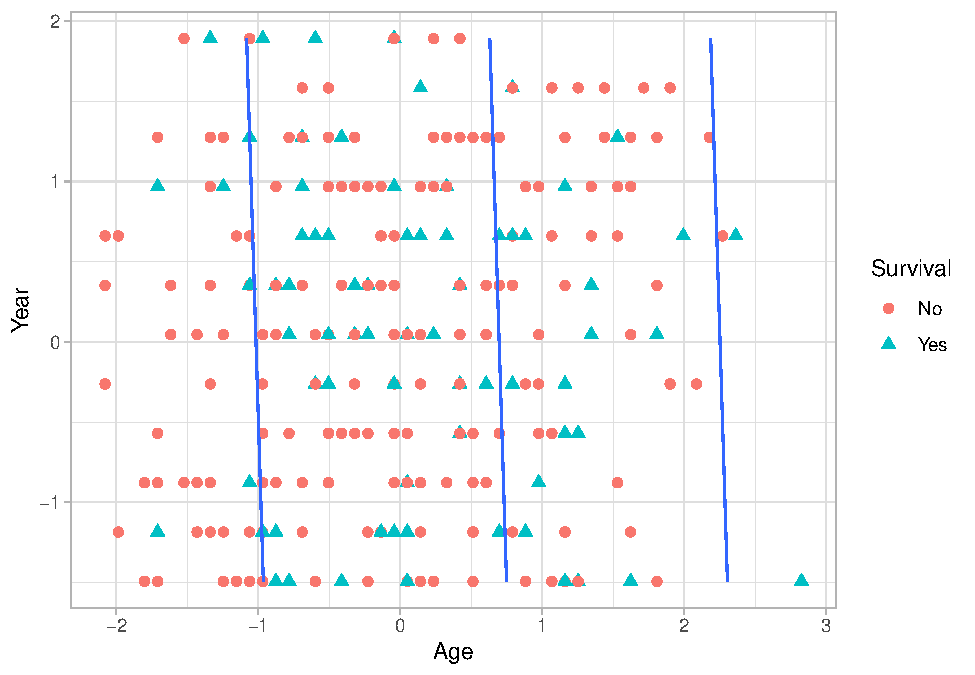
\includegraphics[width=.9\linewidth]{img/Clasificacion_files/figure-latex/unnamed-chunk-26-1}\caption{}\small{Estamos pintando un contorno 3D y por eso nos salen múltiples líneas en el gráfico}\end{figure}

Predecimos en test

\begin{verbatim}
Test evaluation:
Accuracy     Kappa 
0.8709677 0.0000000 

Confusion matrix:
       test_labels
ldaPred No Yes
    No  27   4
    Yes  0   0
\end{verbatim}

Tenemos un dataset bastante desbalanceado, y LDA no predice para la clase Yes. Con esto se asegura un alto accuracy en nuestro entrenamiento, pero no asegura de que para datos externos vaya a ser así. Pese a ello, no nos queda más remedio que suponer que nuestros datos vienen de la misma muestra aleatoria y por tanto son releventes para la clasificación.

\subsection{Algoritmo QDA}
\subsubsection{Asunciones}

QDA tiene las mismas asunciones de LDA salvo que relaja la norma de que las clases tengan igual covarianza. Esto nos permite usar la variable Positive que habíamos descartado en LDA.

\vspace{\baselineskip}

Por tanto tenemos los requisitos de: 
\begin{enumerate}
    \item Distribución aleatoria.
    \item Distribución normal.
\end{enumerate}

Técnicamente el no cumplir normalidad no imposibilita que se encuentre solución, pero ya no nos lo asegura.

\vspace{\baselineskip}

Adicionalmente tenemos de forma recomendada que: 
\begin{itemize}
    \item El número de predictores debe ser menor que el número de instancias de cada clase. 
    
    Del EDA sabemos que esto es cierto.
    \item Los predictores dentro de cada clase no deben estar correlacionados.
    
    Esto podemos verlo mediante matrices de correlación.
\end{itemize}

\begin{figure}[H]\center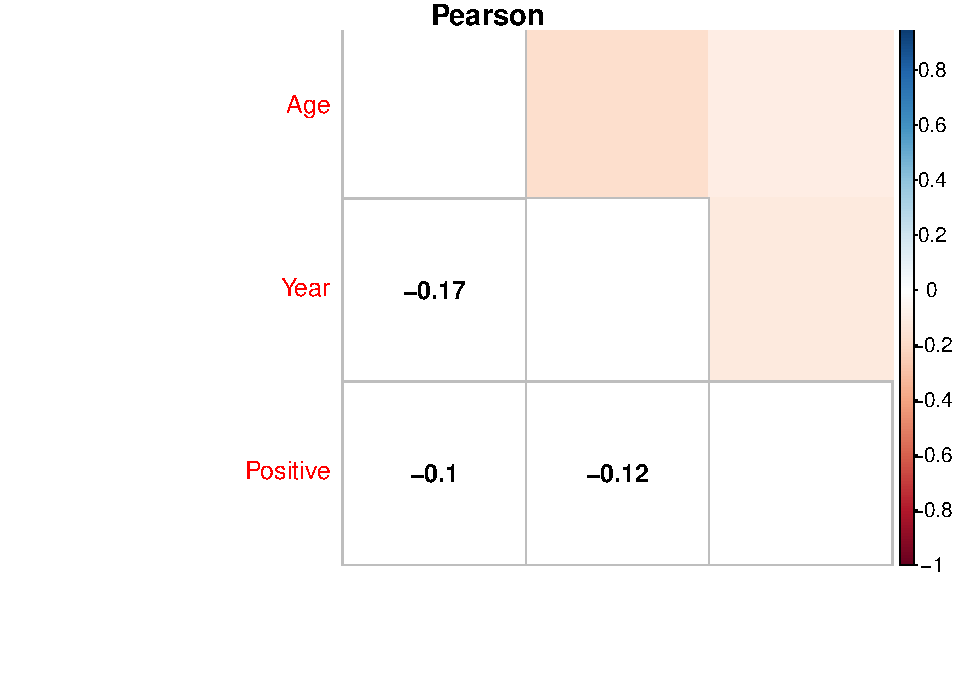
\includegraphics[width=.9\linewidth]{img/Clasificacion_files/figure-latex/unnamed-chunk-27-1}\caption{}\end{figure}

\begin{figure}[H]\center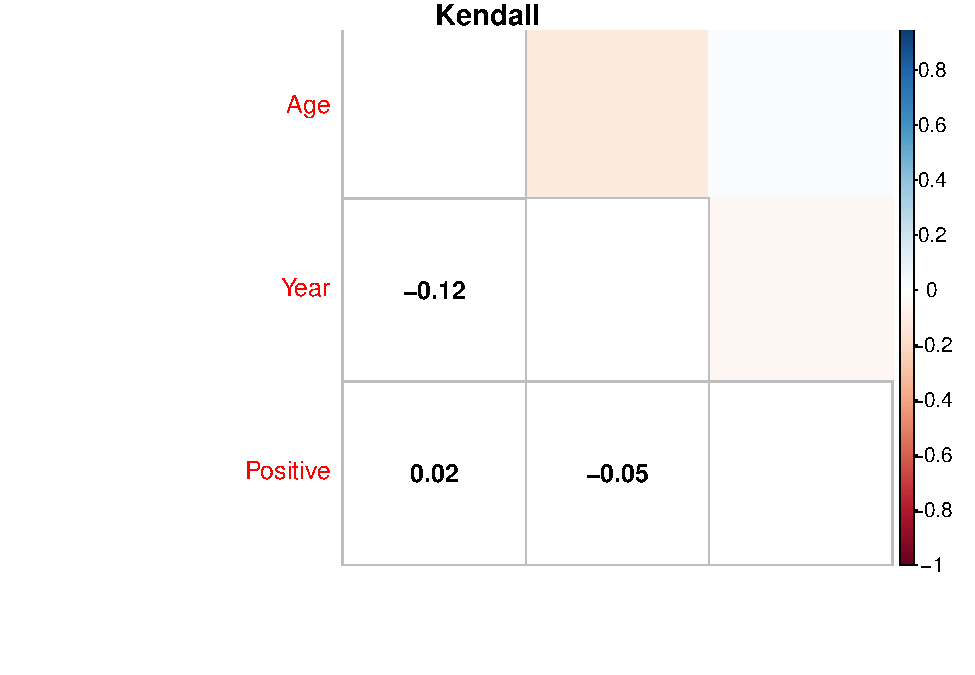
\includegraphics[width=.9\linewidth]{img/Clasificacion_files/figure-latex/unnamed-chunk-27-2}\caption{}\end{figure}

\begin{figure}[H]\center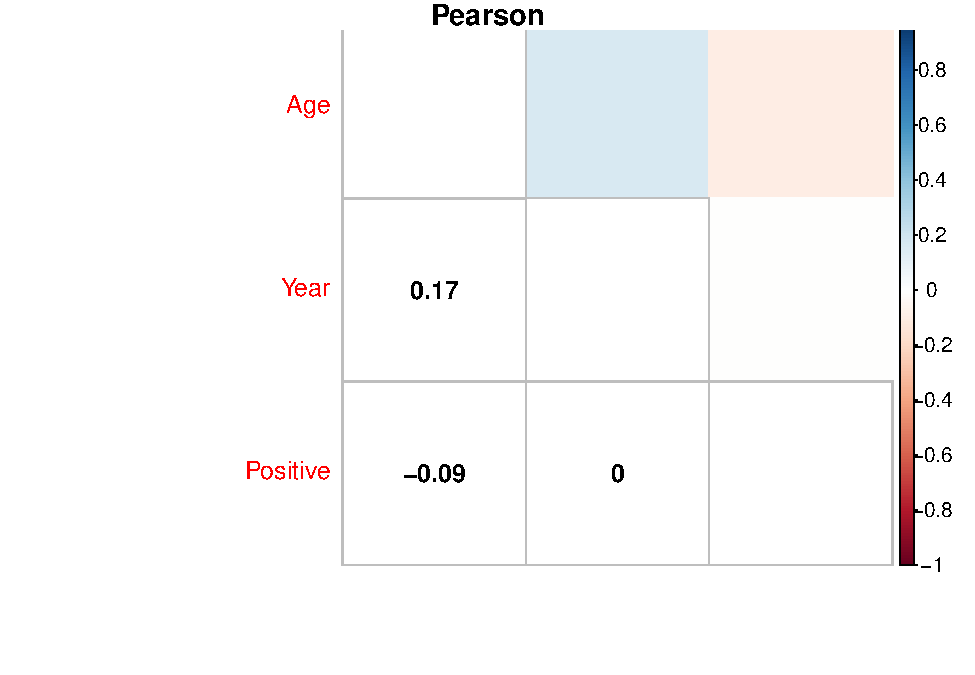
\includegraphics[width=.9\linewidth]{img/Clasificacion_files/figure-latex/unnamed-chunk-28-1}\caption{}\end{figure}

\begin{figure}[H]\center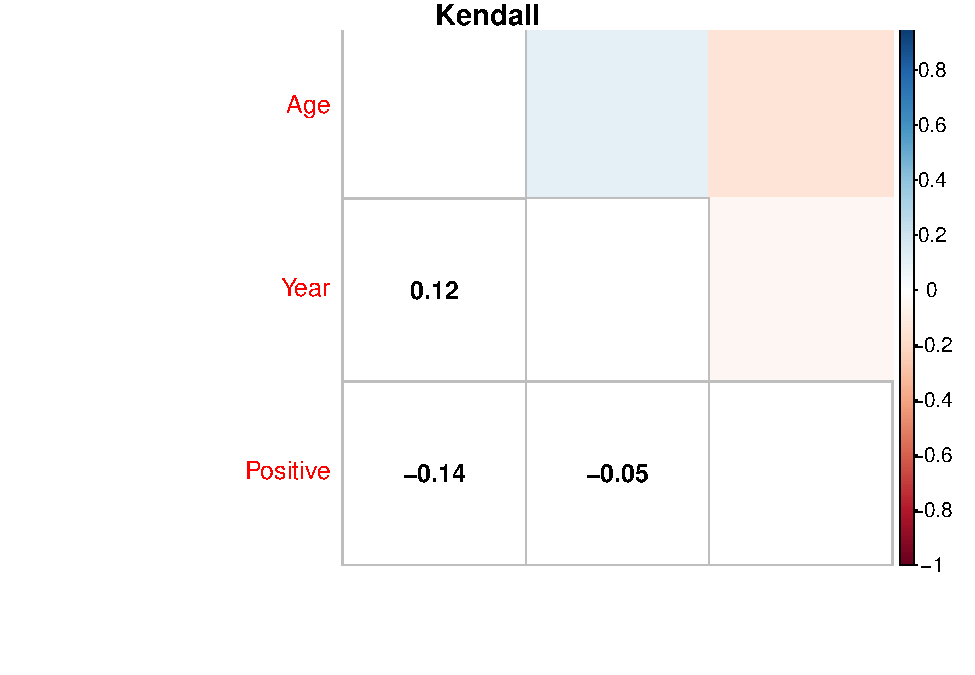
\includegraphics[width=.9\linewidth]{img/Clasificacion_files/figure-latex/unnamed-chunk-28-2}\caption{}\end{figure}

\subsubsection{Aplicación del algoritmo QDA}

\begin{verbatim}
Call:
qda(x, y)

Prior probabilities of groups:
  No  Yes 
0.72 0.28 

Group means:
            Age        Year   Positive
No  -0.04141411 0.004845716 -0.1792534
Yes  0.11031976 0.021276742  0.4804648
Cross-Validated (10 fold) Confusion Matrix 

(entries are percentual average cell counts across resamples)
 
          Reference
Prediction   No  Yes
       No  67.3 21.5
       Yes  4.7  6.5
                            
 Accuracy (average) : 0.7382
\end{verbatim}

\begin{figure}[H]\center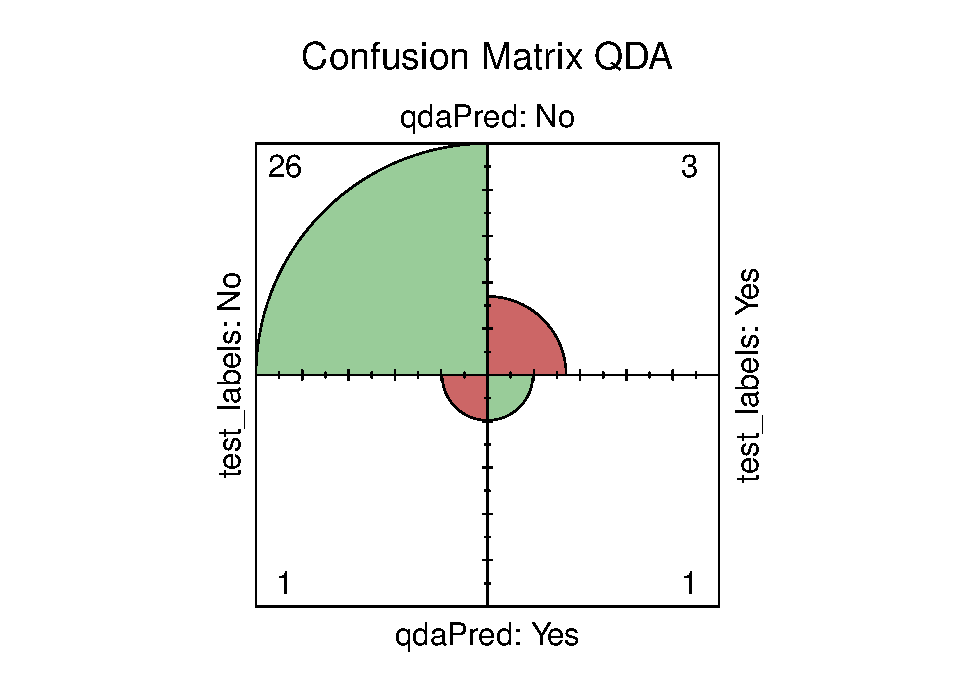
\includegraphics[width=.9\linewidth]{img/Clasificacion_files/figure-latex/unnamed-chunk-31-1}\caption{}\end{figure}

\begin{figure}[H]\center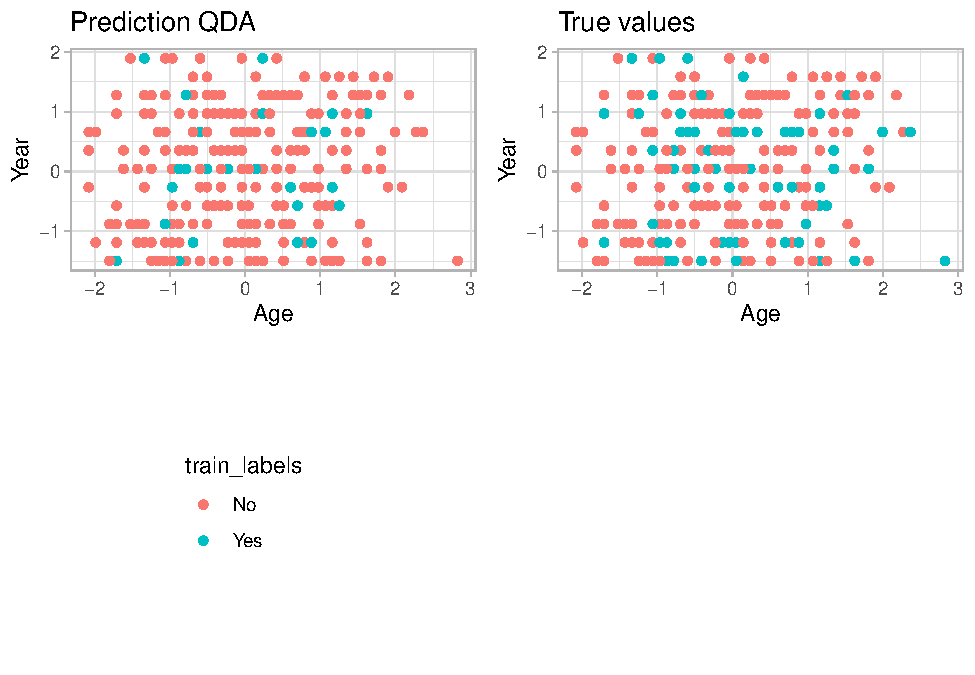
\includegraphics[width=.9\linewidth]{img/Clasificacion_files/figure-latex/unnamed-chunk-32-1}\caption{Predicciones QDA sobre training}\end{figure}


\begin{verbatim}
Test evaluation:
Accuracy     Kappa 
0.8709677 0.2705882

Confusion matrix:
       test_labels
qdaPred No Yes
    No  26   3
    Yes  1   1
\end{verbatim}


Obtenemos resultados extremadamente similares a LDA, pero en este caso vemos que sí se predice la clase Yes.

\subsection{Comparativa de algoritmos}
\subsubsection{Para el dataset \textit{haberman}}

Si nos fijamos únicamente en los resultados obtenidos para este problema, los tres algoritmos obtienen el mismo accuracy en nuestro conjunto de test. Aunque las etiquetas de este conjunto contienen elementos de ambas clases, podemos ver que se predice mayoritariamente la clase \textit{No}. Como se había mencionado nuestro dataset está bastante desbalanceado, por lo que era más probable que se predijera esa clase con mayor facilidad.

\begin{verbatim}
Etiquetas:
No  No  Yes No  No  No  No  No  Yes No  No  No  No  No  No  No  No  Yes No 
No  No  No  No  No  No  No  No  Yes No  No  No 

Predicciones KNN:
No  No  Yes No  No  No  No  Yes No  No  No  No  No  No  No  No  No  Yes No 
No  No  No  No  No  No  No  No  No  No  No  No 

Predicciones LDA:
No No No No No No No No No No No No No No No No No No No No No No No No No
No No No No No No

Predicciones QDA:
No  No  Yes No  No  No  No  Yes No  No  No  No  No  No  No  No  No  No  No 
No  No  No  No  No  No  No  No  No  No  No  No 
\end{verbatim}

\vspace{\baselineskip}

\begin{verbatim}
Accuracy KNN:
 Accuracy     Kappa 
0.9032258 0.5181347 

Accuracy LDA:
 Accuracy     Kappa 
0.8709677 0.0000000 

Accuracy QDA:
 Accuracy     Kappa 
0.8709677 0.2705882 
\end{verbatim}
(Recordamos que las medidas devueltas en cada algoritmo provienen de un CV de 10-fold usando el paquete caret)

Obtenemos valores de accuracy muy similares, pero diferentes valores de Kappa, siendo en general todos bajos.

\vspace{\baselineskip}

Pese a esto, y ya no solo por tener mejores resultados, sino por no cumplir las asunciones necesarias de obtener resultados de calidad en LDA y QDA, para este problema optaríamos por usar el algoritmo KNN.

A partir de las gráficas 3D de las figuras ?? y ?? se apreció una difícil separación de las clases, por lo que el algoritmo de vecinos más cercanos nos resulta una aproximación más lógica.

\subsubsection{Comparativas generales}

Para comparar la calidad genérica de los algoritmos vamos a aplicar test estadísticos en base a los resultados obtenidos en múltiples datasets. Para asegurar la igualdad de condiciones los algoritmos hacen uso de parámetros genéricos y utilizan las mismas particiones de cross-validation.

\vspace{\baselineskip}

Estas son las tablas de resultados que tenemos para test:

\begin{tabular}{l|r|r|r}
\hline
Dataset & out\_test\_knn & out\_test\_lda & out\_test\_qda\\
\hline
appendicitis & 0.8966667 & 0.8690909 & 0.8109091\\
\hline
australian & 0.6838235 & 0.8579710 & 0.8028986\\
\hline
balance & 0.9024546 & 0.8624101 & 0.9167905\\
\hline
bupa & 0.6865775 & 0.6837924 & 0.5991759\\
\hline
contraceptive & 0.5448653 & 0.5091561 & 0.5173102\\
\hline
haberman & 0.7462069 & 0.7481720 & 0.7512903\\
\hline
hayes-roth & 0.5666667 & 0.5500000 & 0.5875000\\
\hline
heart & 0.6692308 & 0.8481481 & 0.8296296\\
\hline
iris & 0.9642857 & 0.9800000 & 0.9733333\\
\hline
led7digit & 0.7510204 & 0.7420000 & 0.6975000\\
\hline
mammographic & 0.7977698 & 0.8241269 & 0.8194042\\
\hline
monk-2 & 0.9743632 & 0.7703433 & 0.9235535\\
\hline
newthyroid & 0.9071429 & 0.9164502 & 0.9629870\\
\hline
pima & 0.7348861 & 0.7709930 & 0.7412403\\
\hline
tae & 0.3838095 & 0.5245833 & 0.5425000\\
\hline
titanic & 0.7850353 & 0.7760304 & 0.7733032\\
\hline
vehicle & 0.6291452 & 0.7813305 & 0.8522409\\
\hline
vowel & 0.6428571 & 0.6030303 & 0.9191919\\
\hline
wine & 0.6959559 & 0.9944444 & 0.9888889\\
\hline
wisconsin & 0.9735023 & 0.9592185 & 0.9519476\\
\hline
\end{tabular}

\vspace{\baselineskip}

Aplicamos el test de Wilcoxon a cada pareja de algoritmos:

\vspace{\baselineskip}

\textbf{LDA vs QDA:} Obtenemos un ranking de 144 para LDA y 96 para QDA, con un p-valor de 0.75 (o nivel de confianza del 25\%).
\begin{verbatim}
V = 96, p-value = 0.7562
alternative hypothesis: true location shift is not equal to 0

  V    V
114 - 96 
\end{verbatim}

Esto nos dice que LDA obtiene mejores resultados pero puesto que el p-value es extremadamente grande no podemos afirmar con garantía estadística que las diferencias entre los tests sean notorias.

\vspace{\baselineskip}

\textbf{LDA vs KNN:} Ahora obtenemos un ranking de 90 para LDA y 120 para QDA, con un p-valor de 0.59 (o nivel de confianza del 41\%).
\begin{verbatim}
V = 120, p-value = 0.5958
alternative hypothesis: true location shift is not equal to 0

 V     V
90 - 120 
\end{verbatim}

Seguimos teniendo un p-valor demasiado grande para poder asegurar la diferencia.

\vspace{\baselineskip}

\textbf{QDA vs KNN:} Por último tenemos un ranking de 69 para LDA y 141 para KNN, con un p-valor de 0.18 (o nivel de confianza del 82\%).
\begin{verbatim}
V = 141, p-value = 0.1893
alternative hypothesis: true location shift is not equal to 0

 V    V
69 - 141
\end{verbatim}

Aunque buscaríamos al menos un 95\% de confianza, podemos afirmar al 82\% que los resultados de ambos algoritmos sí son significativamente diferentes.

\vspace{\baselineskip}
\vspace{\baselineskip}

Una comparativa múltiple de los tres algoritmos con el test de \textbf{Friedman} es la siguiente:

\begin{verbatim}
Friedman rank sum test
Friedman chi-squared = 0.7, 
                  df = 2, 
             p-value = 0.7047
\end{verbatim}

El p-value es mayor que 0.05 por lo que no podemos concluir que haya al menos un par de algoritmos de calidad diferente.

\vspace{\baselineskip}
\vspace{\baselineskip}

Aunque el resultado del test de Friedman ya nos indica que un análisis post-hoc es innecesario, puesto que los resultados que se obtengan no van a asegurar la diferencia en la calidad de los algoritmos, por completitud en la memoria aplicamos el post-hoc de \textbf{Holm}:

\begin{verbatim}
1 = KNN, 2 = LDA, 3 = QDA

Pairwise comparisons using Wilcoxon signed rank exact test 

1    2   
2 1.00 -   
3 0.53 1.00
    
P value adjustment method: holm 
\end{verbatim}

Vemos que los p-value son lo más altos posibles, por lo que carece de sentido intentar diferenciar los algoritmos. Aunque podemos notar, tal y como habíamos visto en los test de Wilcoxon, que la diferencia KNN-QDA probablemente sea mayor que el resto de parejas.